\chapter{An Example}
This section will present a pedagogically interesting 
example which demonstrates several of the program's important
features.  The purpose of this chapter is neither to be 
comprehensive nor to be particularly detailed. It will instead 
give a sense of the types of analysis that can be done with 
this program. It will act as a motivation for the rest of the manual. 
Further details 
and information on any of the things described below can be found in 
the appropriate sections of the manual.

David, a user of the program, was studying iron thin films 
using powder diffraction. He was particularly interested in 
measuring the shift in diffraction peaks of his sample. To 
realize this experimentally, he capture data of the 
standard calibration crystal Lanthanum Hexaboride (LaB6). 
Without changing the experimental parameters, he then imaged 
many samples that he wanted to analyze. 

The steps that are needed to do this analysis will be
described. The diffraction detector needs to first be calibrated.
This will determine the precise experimental parameters that 
characterize the diffraction machine when the data was captured
(for example, the distance between sample and detector, the energy 
of the x-rays, etc). Since the image of the standard was taken at the same
time as the other images, the calibration parameters inferred
from the standard crystal can be used to analyze the
rest of data.

\begin{SCfigure}[1][bthp]
    \centering
    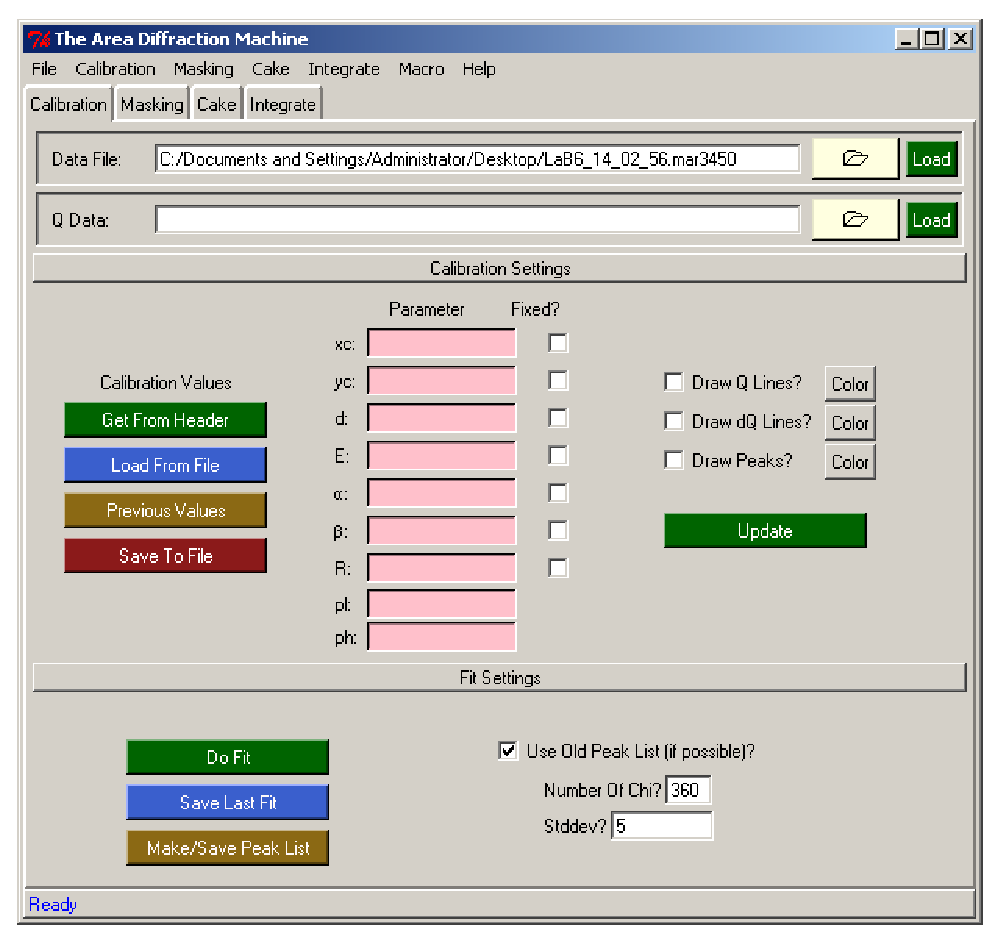
\includegraphics[scale=.75]
    {figures/calibration_tab.eps}
    \caption{The calibration tab.}
    \label{calibration_tab_example}
\end{SCfigure}

To perform this calibration, the Area Diffraction Machine needs 
to be opened. Figure~\ref{calibration_tab_example} shows what 
is first displayed. Using the \gui{Data File} input, the LaB6
file can be loaded.. A new window opens up which shows the 
diffraction data. This window is shown in 
figure~\ref{diffraction_data_window_example}.

\begin{SCfigure}[1][bthp]
    \centering
    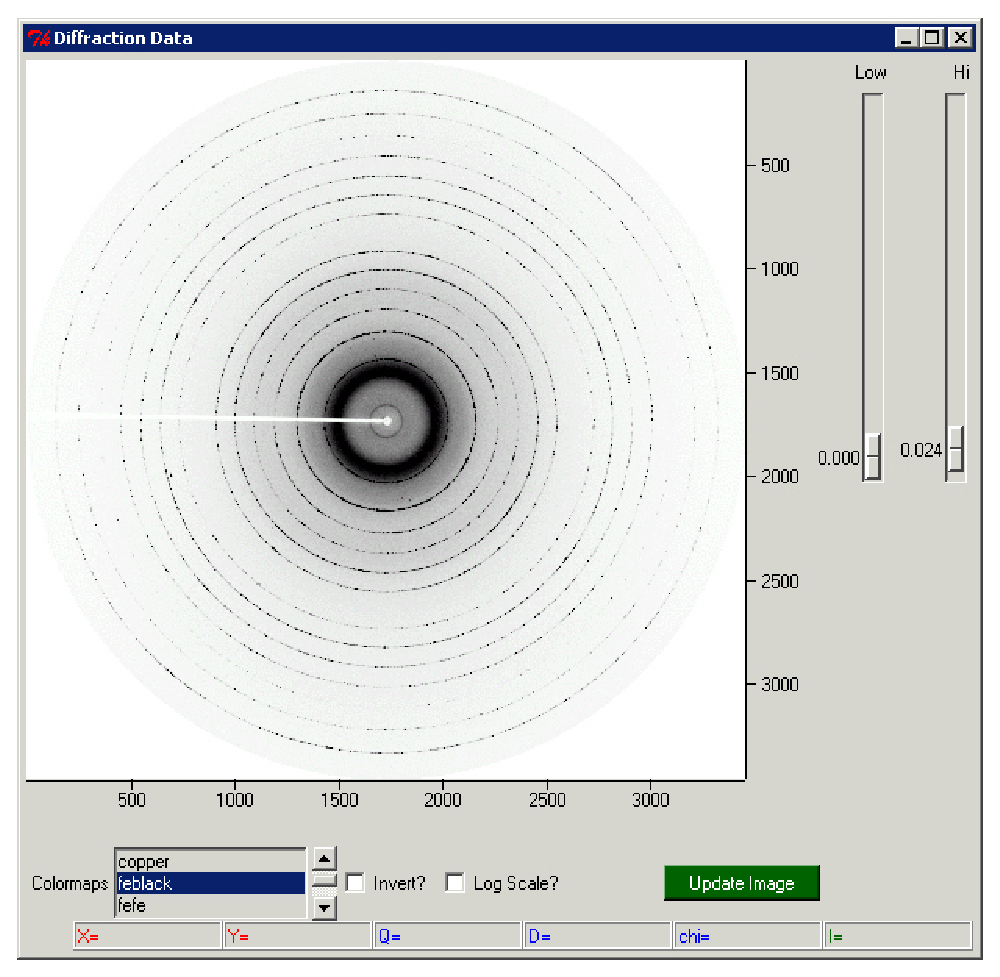
\includegraphics[scale=.75]
    {figures/diffraction_data_window_example.eps}
    \caption{The diffraction data window.}
    \label{diffraction_data_window_example}
\end{SCfigure}

To calibrate the detector, the program must know the 
$Q$ values for the standard crystal. Since LaB6 is so common, it is
a preset default in the program. It can be loaded from
the \gui{Standard Q} option in the \gui{Calibration} menu.
This is shown in figure~\ref{standard_q_example}.

\begin{SCfigure}[1][bthp]
    \centering
    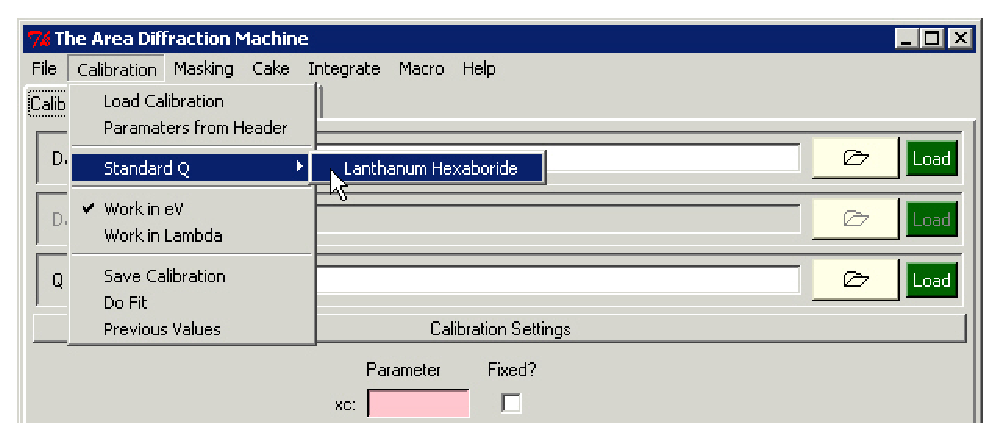
\includegraphics[scale=.75]
    {figures/standard_q.eps}
    \caption{Loading a standard $Q$ file.
    (More standard $Q$ files might be added in the future).}
    \label{standard_q_example}
\end{SCfigure}

In order to calibration the detector, the program also
needs an initial guess of the calibration parameters. 
Decent guesses at the experimental parameters are often
stored in the diffraction data's header. 
The program can try to find these header calibration values 
and put them into the program. This is done with the
\gui{Get From Header} button. After the image, the $Q$ values, 
and an initial guess at the parameters have been loaded, 
The detector can be calibrated.

But first, it is a good practice to examine how good the 
initial guess is. This is be done with the \gui{Draw Q Lines?}
check box on the \gui{Calibration} tab. When this is selected, 
the program will draw
on top of the diffraction image what pattern should show 
up on the detector (for the given calibration parameters and $Q$
values). Figure~\ref{bad_calibration_diffraction_image}
shows an example. Of course, the initial guess isn't
great because the lines don't match the real pattern.

\begin{SCfigure}[1][bthp]
    \centering
    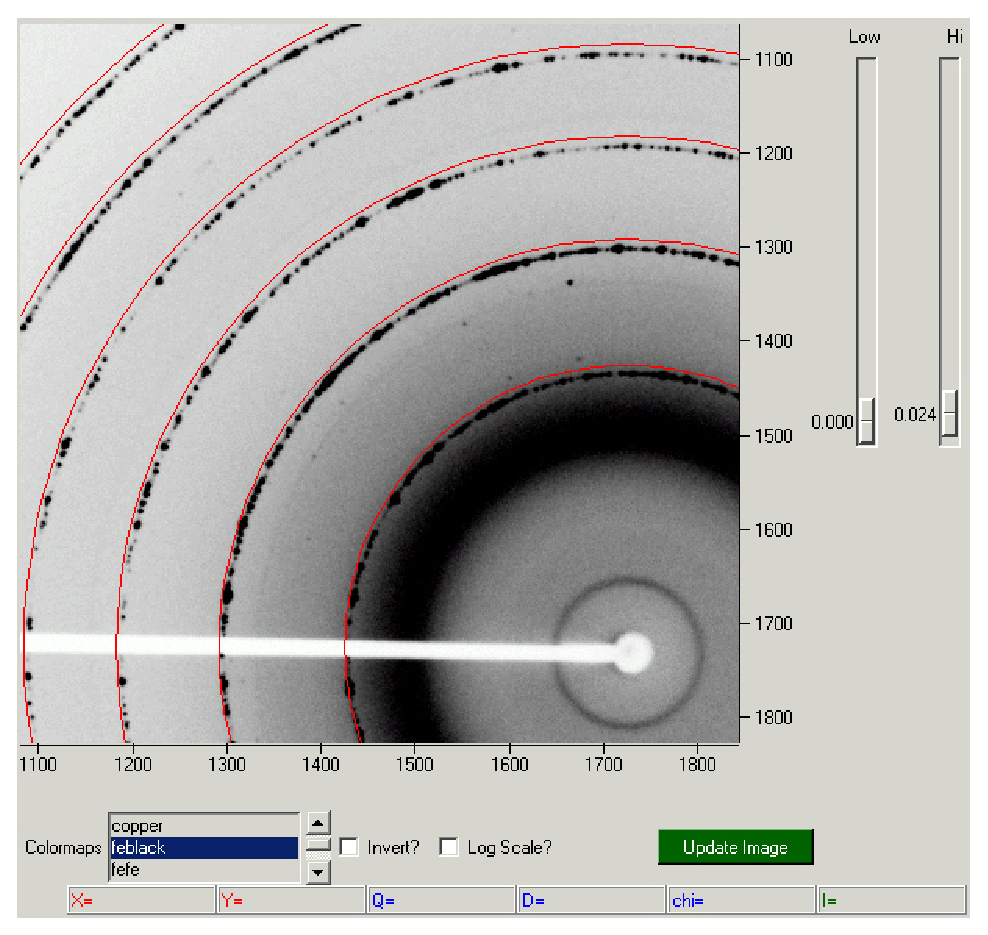
\includegraphics[scale=.75]
    {figures/bad_calibration_diffraction_image.eps}
    \caption{The diffraction image with constant $Q$
    lines displayed on it. These lines were calculated
    for the calibration parameters found in the
    image header and are not particularly accurate.}
    \label{bad_calibration_diffraction_image}
\end{SCfigure}

The diffraction data can be caked. A cake is a plot
of the data in $Q$ vs. $\chi$ space. 
If the calibration parameters are known exactly, 
the diffraction peaks will show up as many vertical lines.
If the parameters are not exact, the diffraction peaks
will have a distortion to them.
The data can be caked on the \gui{Cake} tab using the 
\gui{AutoCake} button and a new window will open. 
this tab is shown in figure~\ref{cake_tab_example} 
and the cake window is shown in 
figure~\ref{bad_calibration_cake}.
The diffraction peaks on the caked data with the header 
calibration parameters is not very straight. It has a 
systematic wiggle. It might be hard to see 
with the full image but is very obvious when one line
is zoomed into, as in 
figure~\ref{bad_calibration_cake_zoom}.


\begin{SCfigure}[1][bthp]
    \centering
    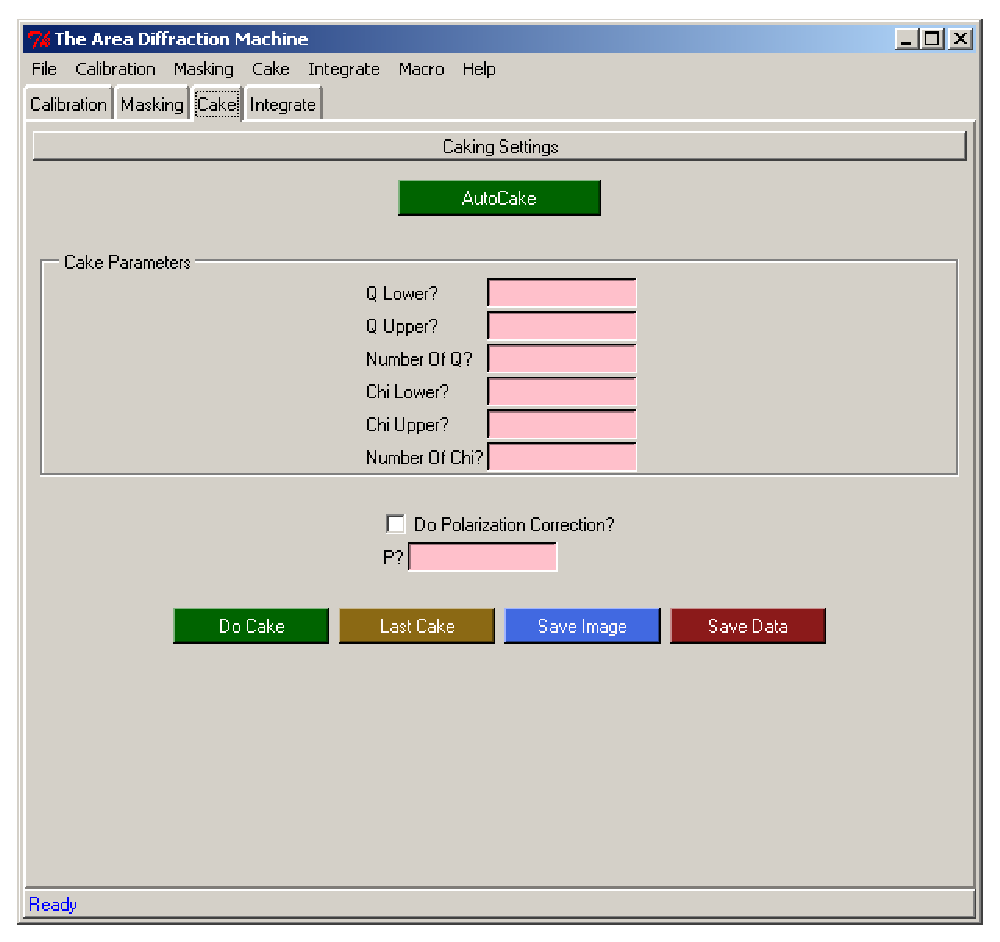
\includegraphics[scale=.75]
    {figures/caking_tab.eps}
    \caption{The calibration tab.}
    \label{cake_tab_example}
\end{SCfigure}

\begin{SCfigure}[1][bthp]
    \centering
    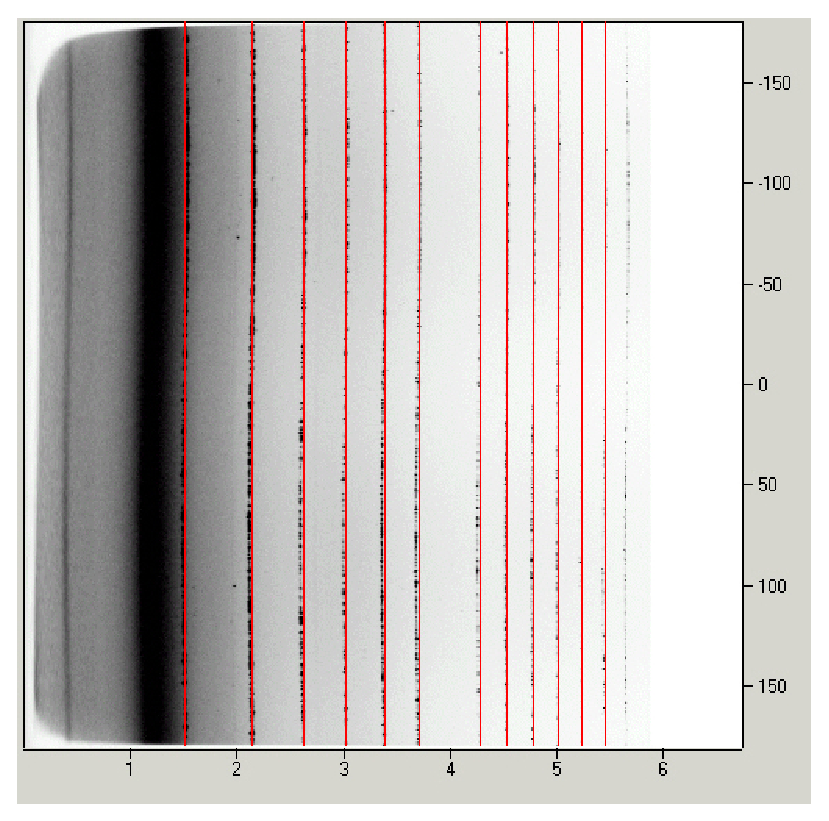
\includegraphics[scale=.75]
    {figures/bad_calibration_cake.eps}
    \caption{A cake done with the calibration parameters
    found in the image header. These parameters
    are not particularly good and the diffraction peaks
    are not very straight. Calibration improves
    the straightness of these peaks.}
    \label{bad_calibration_cake}
\end{SCfigure}

\begin{SCfigure}[1][bthp]
    \centering
    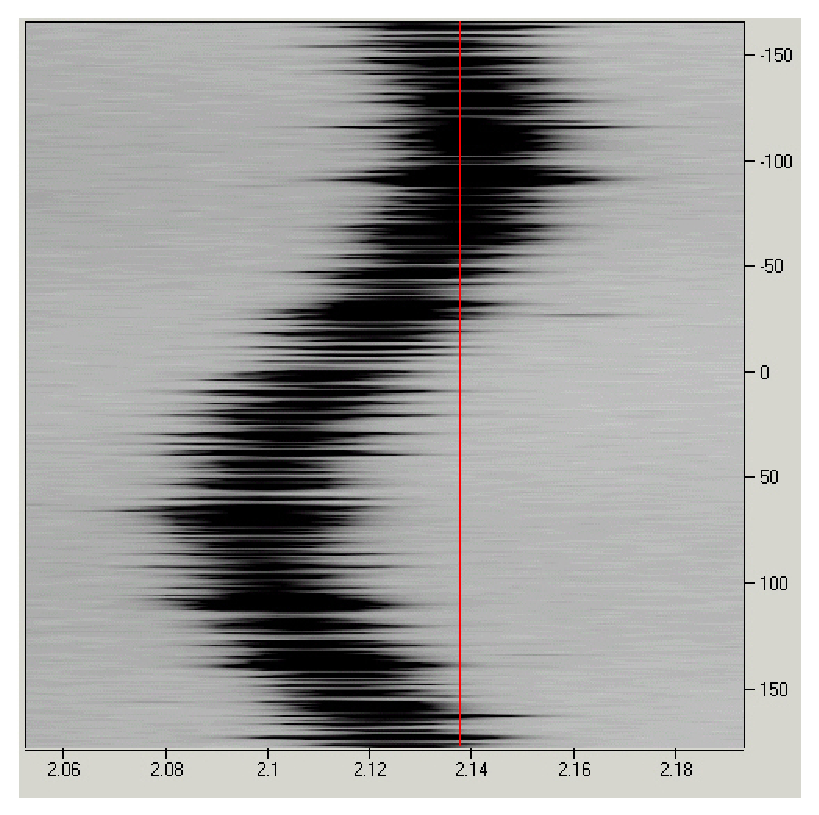
\includegraphics[scale=.75]
    {figures/bad_calibration_cake_zoom.eps}
    \caption{A zoom in of the cake shown in 
    figure~\ref{bad_calibration_cake}. When zoomed into 
    diffraction image, the poor calibration becomes much 
    more obvious.}
    \label{bad_calibration_cake_zoom}
\end{SCfigure}

Calibration can be done to improve the experimental
parameters. It is done with the \gui{Do Fit} button 
on the \gui{Calibration} tab. If the calibration is good, 
the constant $Q$ lines drawn on the diffraction image 
entirely overlap the real diffraction patter. 
This is shown in figure~\ref{good_calibration_diffraction_image}.
The peaks on the caked image also become much straighter.
The caked data after calibration is shown in 
figure~\ref{good_calibration_cake}.
figure~\ref{good_calibration_cake_zoom} shows that they
look good even when zoomed in.

\begin{SCfigure}[1][bthp]
    \centering
    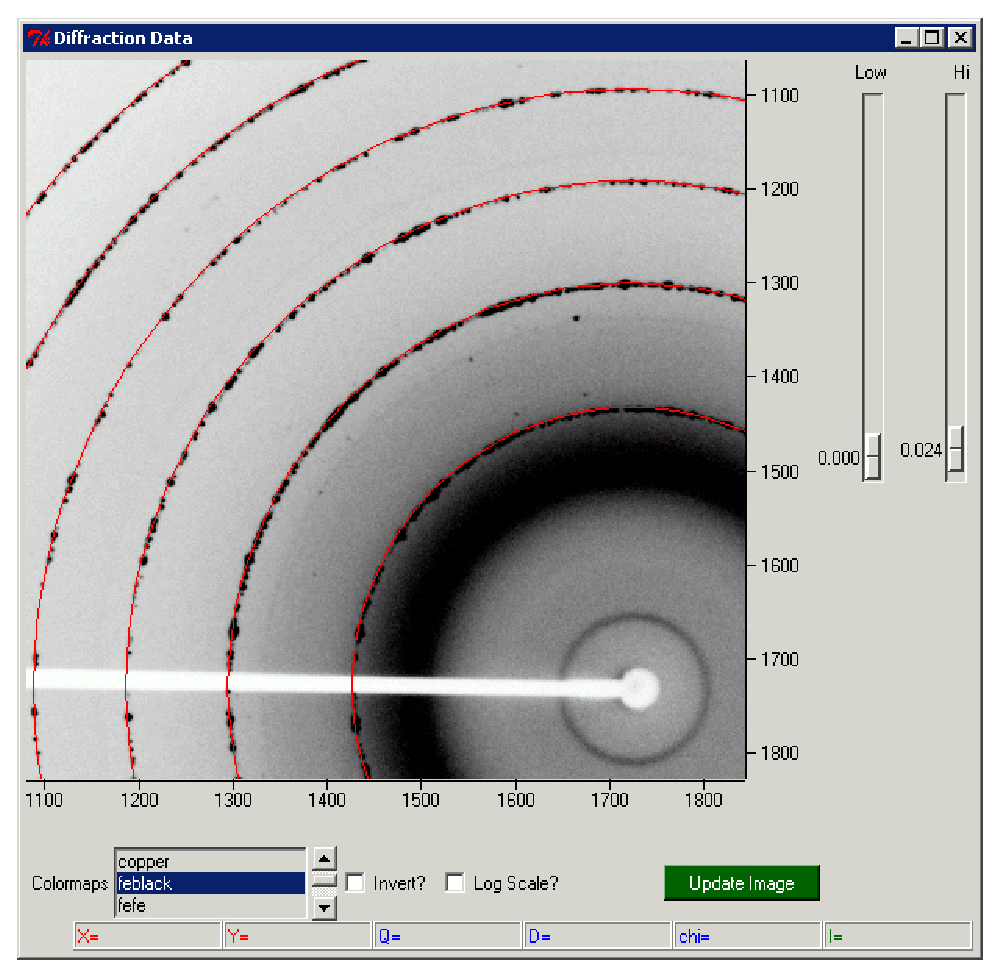
\includegraphics[scale=.75]
    {figures/good_calibration_diffraction_image.eps}
    \caption{The diffraction window after being calibrated. The
    constant $Q$ lines fall well on top of the diffraction 
    peaks.}
    \label{good_calibration_diffraction_image}
\end{SCfigure}

\begin{SCfigure}[1][bthp]
    \centering
    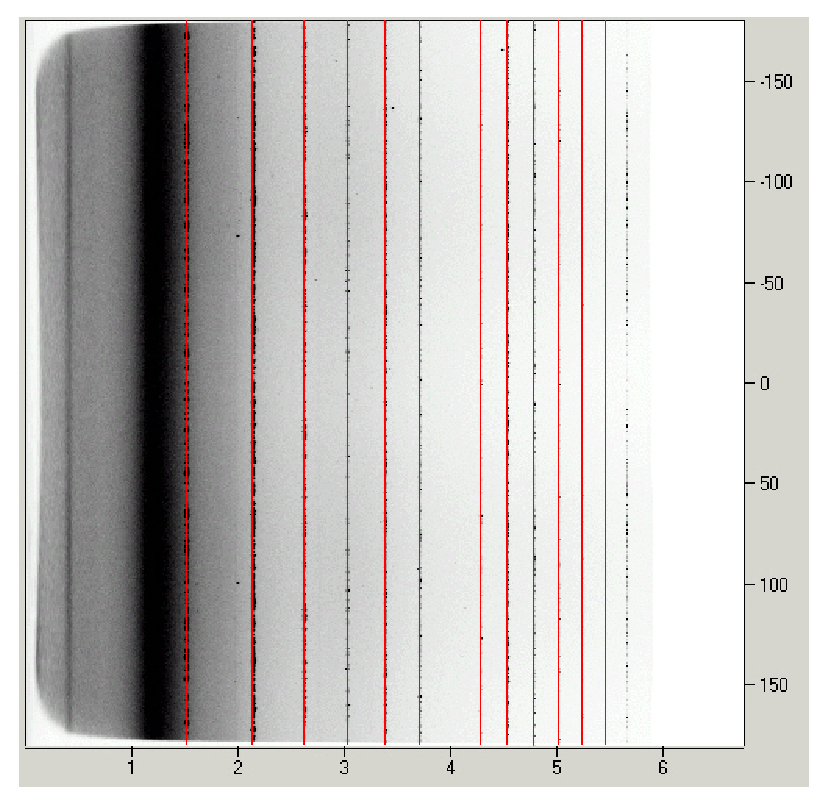
\includegraphics[scale=.75]
    {figures/good_calibration_cake.eps}
    \caption{The cake window after calibration.  The lines 
    are much straighter than the lines in 
    figure~\ref{bad_calibration_cake} before calibration.}
    \label{good_calibration_cake}
\end{SCfigure}

\begin{SCfigure}[1][bthp]
    \centering
    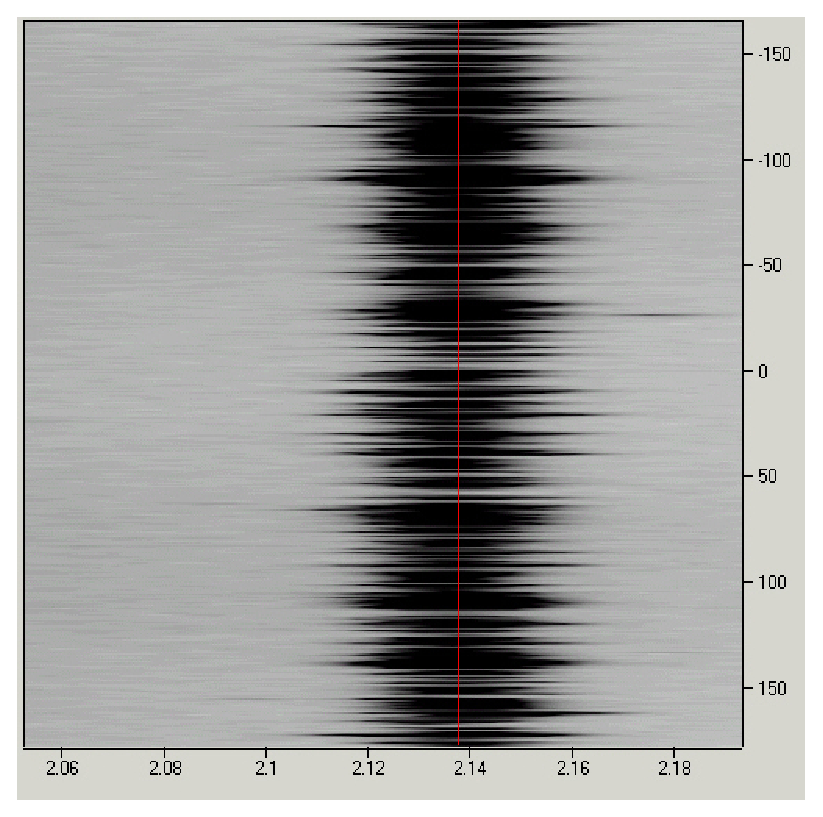
\includegraphics[scale=.75]
    {figures/good_calibration_cake_zoom.eps}
    \caption{A zoomed in part of figure~\ref{good_calibration_cake}. 
    Even at a large zoom in, the line remains very straight.}
    \label{good_calibration_cake_zoom}
\end{SCfigure}

After calibration, the calibration parameters can be saved to 
a file for later use using the \gui{Save to File} button on the 
\gui{Calibration} tab. The calibration parameters gets saved as
\begin{lstlisting}[caption={'C:/Data/LaB6\_cal.dat'}]
xc	1722.966078	0
yc	1724.227970	0
D	122.691351	0
E	12707.219316	0
alpha	-0.052910	0
beta	0.130553	0
rotation	-41.523477	0
pixelLength	100.000000
pixelHeight	100.000000
\end{lstlisting}

As figure~\ref{diffraction_data_window_example} shows,
there is a beam stop in the image obstructing part of the data. 
None of the pixels blocked by the beam stop are part of the interference
pattern so they should be ignored. They can be ignored with a polygon mask
on the \gui{masking} tab. The masking tab is shown in 
figure~\ref{masking_tab_example}. A rectangular mask is 
put on top of the beam stop. The diffraction image with
the mask is shown in
figure~\ref{masked_beam_stop}.
The \gui{Save Mask} button can be used to save the mask
to a file. The saved file is
\begin{lstlisting}[caption={'beam\_stop\_mask.dat'}]
# Polygon(s) drawn on Mon Apr 14 00:33:12 2008
25.6749379653	1634.63771712
42.7915632754	1814.36228288
1959.85359801	1857.15384615
1959.85359801	1626.07940447
\end{lstlisting}
This mask can be loaded into the program later when
doing the rest of the analysis.

\begin{SCfigure}[1][bthp]
    \centering
    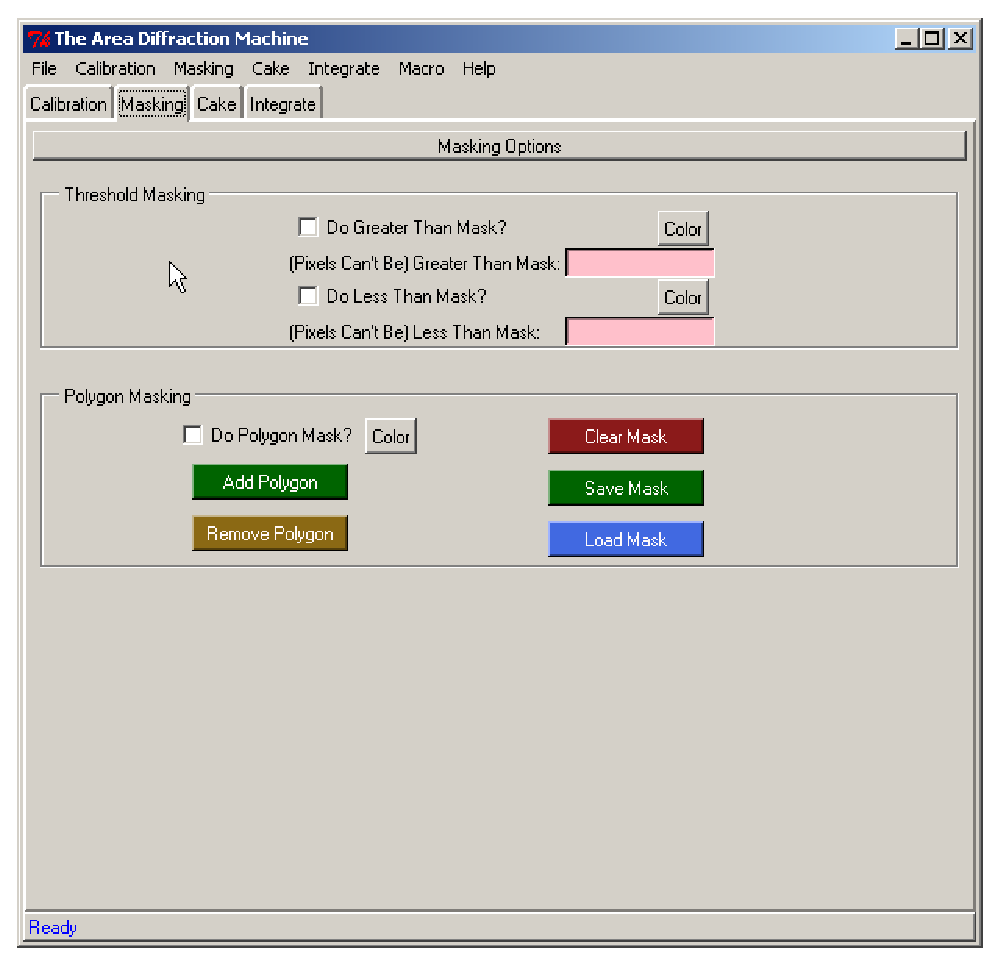
\includegraphics[scale=.75]
    {figures/masking_tab.eps}
    \caption{The pixel masking tab.}
    \label{masking_tab_example}
\end{SCfigure}

\begin{SCfigure}[1][bthp]
    \centering
    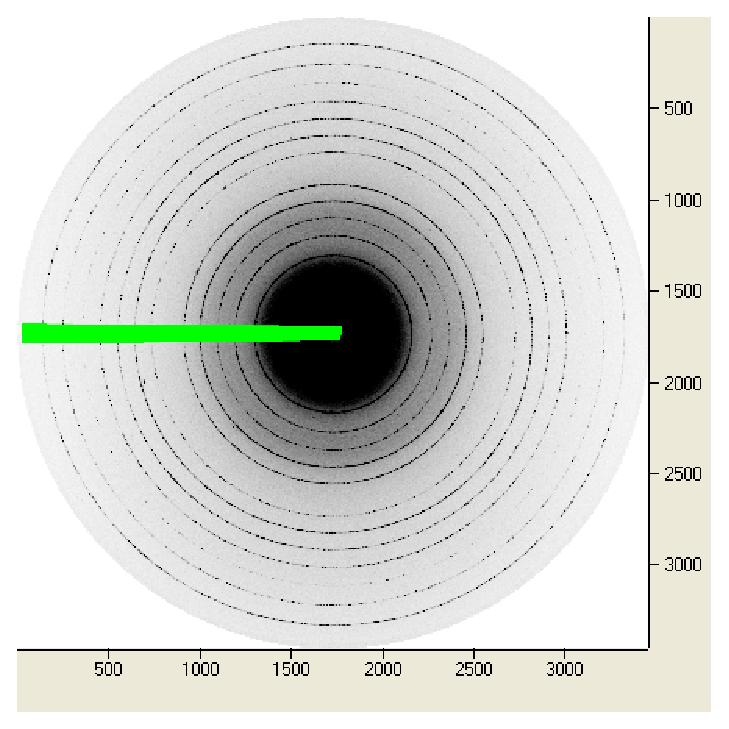
\includegraphics[scale=.75]
    {figures/masked_beam_stop.eps}
    \caption{THis is the same data that is in
    figure~\ref{diffraction_data_window_example} with a
    mask drawn over the beam stop. The mask will ensure
    that the beam stop will not be used in subsequent analysis.}
    \label{masked_beam_stop}
\end{SCfigure}

After calibrating the detector and creating the beam stop mask, 
the rest of the data can be analyzed. This is done by 
performing an intensity integration on each of the other files.
The intensity integrated data is what contains the diffraction peaks.
To perform the integration, the diffraction file must first be loaded.
The calibration parameters determined earlier must be loaded and the
beam stop mask must be loaded using the \gui{Load Mask} button on the
\gui{Masking} tab. The \gui{Do Polygon Mask?} check box needs to
be selected to ensure that the polygon masks are used in the analysis.
Then, a $Q-I$ integration is done by going to the \gui{Integration} tab
and pushing the \gui{AutoIntegrate} button on the left side of the tab.
This is shown in figure~\ref{integration_tab_example}.
One of the iron samples is shown in figure~\ref{iron_intensity}.

\begin{SCfigure}[1][bthp]
    \centering
    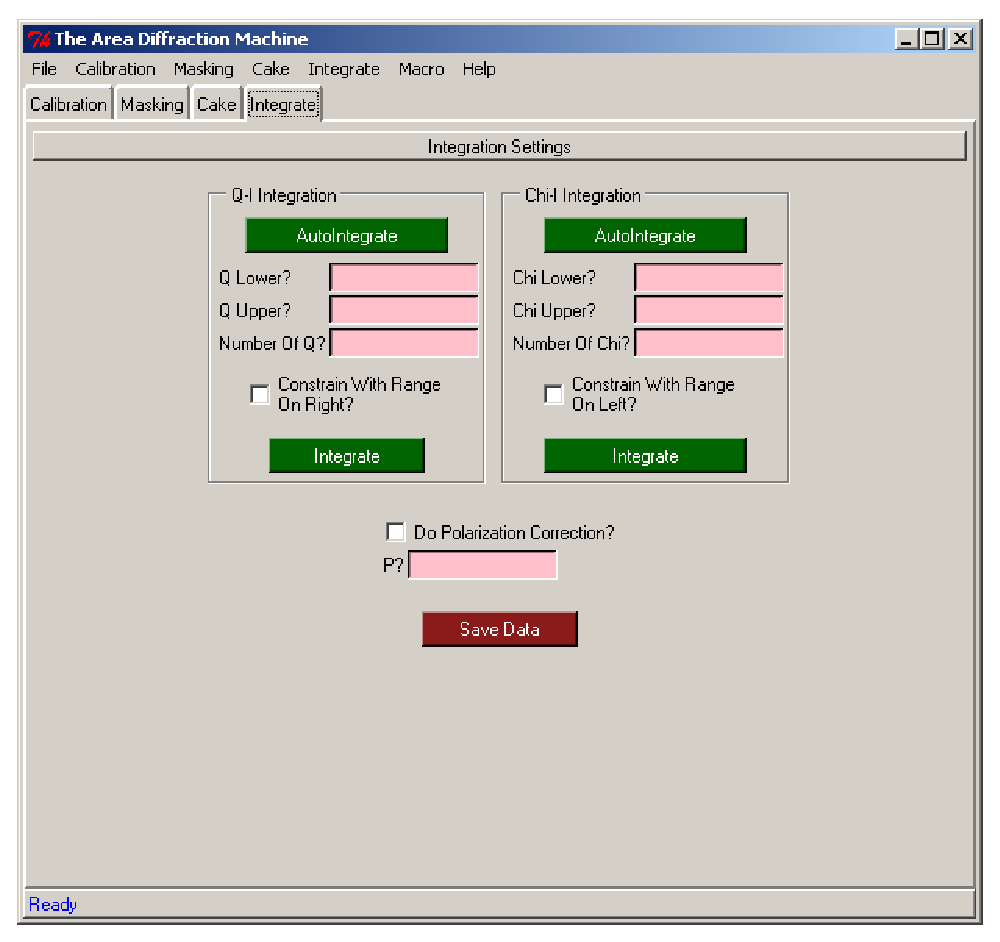
\includegraphics[scale=.75]
    {figures/integration_tab.eps}
    \caption{The integration tab.}
    \label{integration_tab_example}
\end{SCfigure}

\begin{SCfigure}[1][bthp]
    \centering
    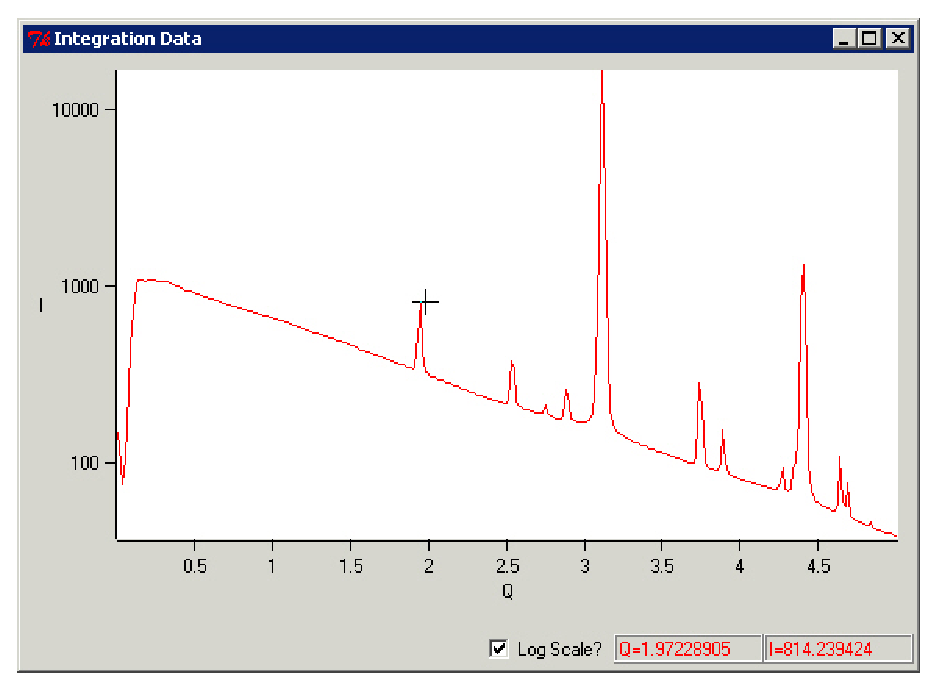
\includegraphics[scale=.75]
    {figures/iron_intensity.eps}
    \caption{The intensity integration window for 
    a particular iron sample.}
    \label{iron_intensity}
\end{SCfigure}

The intensity integrated data can be saved to a file
using the \gui{Save Data} button on the \gui{Integration} tab. 
The data is saved out as two column ASCII. This same 
process could be done to all the files that need to be 
analyzed but if there were a lot of files to analyze, this 
process would be very time consuming. If all of the data was in 
the folder \macroline{C:/Data/}, all the data could be analyzed by 
running the macro
\begin{lstlisting}[caption={'A macro to automate the 
    analysis'}]
Data File:
	C:/Data/
Load From File
    C:/Data/LaB6_cal.dat
Load Mask
    C:/Data/beam_stop_mask.dat
Do Polygon Mask?
    Select
AutoIntegrate Q-I
Save Integration Data
    PATHNAME/FILENAME_int.dat
\end{lstlisting}
The first command loads into the program all the
diffraction files in the folder \macroline{C:/Data/}
one at a time and runs the rest of the analysis on
each of them. The macro loads in the calibration parameters
that were saved earlier and then loads in the beam stop 
mask. The program then does a $Q-I$ intensity integration and 
saves the integration data to a file. The PATHNAME keyword gets
replaced with the path leading up to the particular 
file and the FILENAME keyword gets replaced with 
the particular diffraction file's name. For example, the file
\macroline{FeL2\_d070.mar3450} in
the folder \macroline{C:/Data/} would
be replaced with
\macroline{C:/Data/FeL2\_d070\_int.dat}
This command saves out the intensity integrated data next 
to the corresponding diffraction file with a useful name.

After the macro is run, all the data will be analyzed. The
intensity integrated data can be open in Excel. 
The diffraction patterns of different data can be plotted on
the same graph to look for shifts in teh diffraction peaks. 
This data would look something like the graph shown
in figure~\ref{excel_peak_shift}.

\begin{SCfigure}[1][bthp]
    \centering
    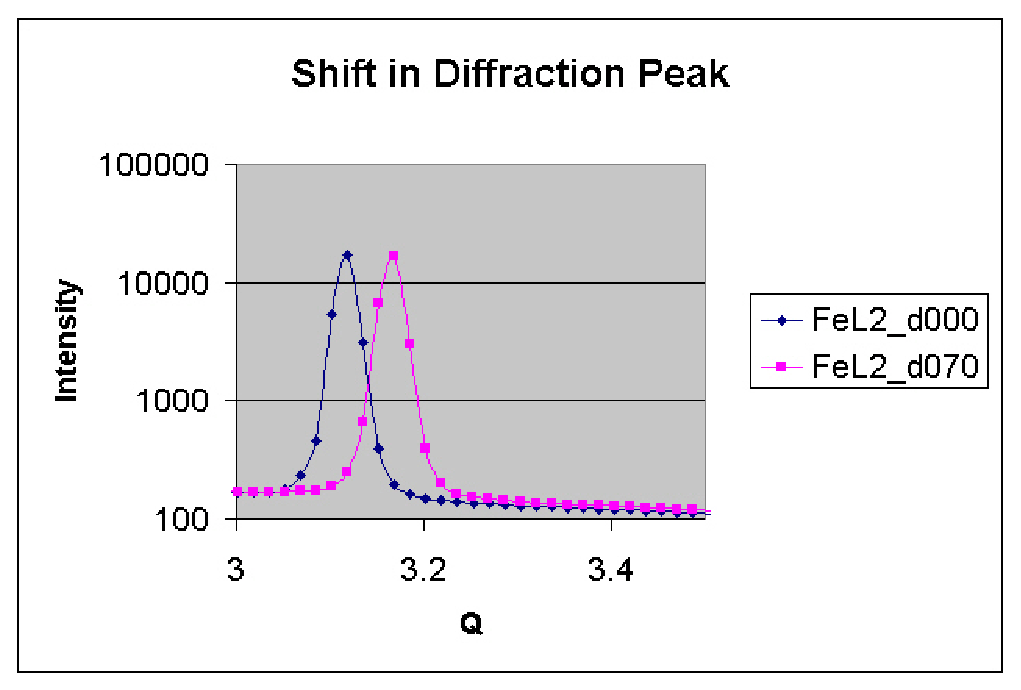
\includegraphics[scale=.5]
    {figures/excel_peak_shift.eps}
    \caption{An example of what the shift in peaks might
    look like when two diffraction patterns were plotted
    in Excel on top of one another.}
    \label{excel_peak_shift}
\end{SCfigure}
